\documentclass[]{article}
\usepackage{lmodern}
\usepackage{amssymb,amsmath}
\usepackage{ifxetex,ifluatex}
\usepackage{fixltx2e} % provides \textsubscript
\ifnum 0\ifxetex 1\fi\ifluatex 1\fi=0 % if pdftex
  \usepackage[T1]{fontenc}
  \usepackage[utf8]{inputenc}
\else % if luatex or xelatex
  \ifxetex
    \usepackage{mathspec}
  \else
    \usepackage{fontspec}
  \fi
  \defaultfontfeatures{Ligatures=TeX,Scale=MatchLowercase}
\fi
% use upquote if available, for straight quotes in verbatim environments
\IfFileExists{upquote.sty}{\usepackage{upquote}}{}
% use microtype if available
\IfFileExists{microtype.sty}{%
\usepackage{microtype}
\UseMicrotypeSet[protrusion]{basicmath} % disable protrusion for tt fonts
}{}
\usepackage[margin=1in]{geometry}
\usepackage{hyperref}
\hypersetup{unicode=true,
            pdftitle={Simulation of Revenue Distribution in R language. Process Reveal.},
            pdfborder={0 0 0},
            breaklinks=true}
\urlstyle{same}  % don't use monospace font for urls
\usepackage{color}
\usepackage{fancyvrb}
\newcommand{\VerbBar}{|}
\newcommand{\VERB}{\Verb[commandchars=\\\{\}]}
\DefineVerbatimEnvironment{Highlighting}{Verbatim}{commandchars=\\\{\}}
% Add ',fontsize=\small' for more characters per line
\usepackage{framed}
\definecolor{shadecolor}{RGB}{248,248,248}
\newenvironment{Shaded}{\begin{snugshade}}{\end{snugshade}}
\newcommand{\AlertTok}[1]{\textcolor[rgb]{0.94,0.16,0.16}{#1}}
\newcommand{\AnnotationTok}[1]{\textcolor[rgb]{0.56,0.35,0.01}{\textbf{\textit{#1}}}}
\newcommand{\AttributeTok}[1]{\textcolor[rgb]{0.77,0.63,0.00}{#1}}
\newcommand{\BaseNTok}[1]{\textcolor[rgb]{0.00,0.00,0.81}{#1}}
\newcommand{\BuiltInTok}[1]{#1}
\newcommand{\CharTok}[1]{\textcolor[rgb]{0.31,0.60,0.02}{#1}}
\newcommand{\CommentTok}[1]{\textcolor[rgb]{0.56,0.35,0.01}{\textit{#1}}}
\newcommand{\CommentVarTok}[1]{\textcolor[rgb]{0.56,0.35,0.01}{\textbf{\textit{#1}}}}
\newcommand{\ConstantTok}[1]{\textcolor[rgb]{0.00,0.00,0.00}{#1}}
\newcommand{\ControlFlowTok}[1]{\textcolor[rgb]{0.13,0.29,0.53}{\textbf{#1}}}
\newcommand{\DataTypeTok}[1]{\textcolor[rgb]{0.13,0.29,0.53}{#1}}
\newcommand{\DecValTok}[1]{\textcolor[rgb]{0.00,0.00,0.81}{#1}}
\newcommand{\DocumentationTok}[1]{\textcolor[rgb]{0.56,0.35,0.01}{\textbf{\textit{#1}}}}
\newcommand{\ErrorTok}[1]{\textcolor[rgb]{0.64,0.00,0.00}{\textbf{#1}}}
\newcommand{\ExtensionTok}[1]{#1}
\newcommand{\FloatTok}[1]{\textcolor[rgb]{0.00,0.00,0.81}{#1}}
\newcommand{\FunctionTok}[1]{\textcolor[rgb]{0.00,0.00,0.00}{#1}}
\newcommand{\ImportTok}[1]{#1}
\newcommand{\InformationTok}[1]{\textcolor[rgb]{0.56,0.35,0.01}{\textbf{\textit{#1}}}}
\newcommand{\KeywordTok}[1]{\textcolor[rgb]{0.13,0.29,0.53}{\textbf{#1}}}
\newcommand{\NormalTok}[1]{#1}
\newcommand{\OperatorTok}[1]{\textcolor[rgb]{0.81,0.36,0.00}{\textbf{#1}}}
\newcommand{\OtherTok}[1]{\textcolor[rgb]{0.56,0.35,0.01}{#1}}
\newcommand{\PreprocessorTok}[1]{\textcolor[rgb]{0.56,0.35,0.01}{\textit{#1}}}
\newcommand{\RegionMarkerTok}[1]{#1}
\newcommand{\SpecialCharTok}[1]{\textcolor[rgb]{0.00,0.00,0.00}{#1}}
\newcommand{\SpecialStringTok}[1]{\textcolor[rgb]{0.31,0.60,0.02}{#1}}
\newcommand{\StringTok}[1]{\textcolor[rgb]{0.31,0.60,0.02}{#1}}
\newcommand{\VariableTok}[1]{\textcolor[rgb]{0.00,0.00,0.00}{#1}}
\newcommand{\VerbatimStringTok}[1]{\textcolor[rgb]{0.31,0.60,0.02}{#1}}
\newcommand{\WarningTok}[1]{\textcolor[rgb]{0.56,0.35,0.01}{\textbf{\textit{#1}}}}
\usepackage{longtable,booktabs}
\usepackage{graphicx,grffile}
\makeatletter
\def\maxwidth{\ifdim\Gin@nat@width>\linewidth\linewidth\else\Gin@nat@width\fi}
\def\maxheight{\ifdim\Gin@nat@height>\textheight\textheight\else\Gin@nat@height\fi}
\makeatother
% Scale images if necessary, so that they will not overflow the page
% margins by default, and it is still possible to overwrite the defaults
% using explicit options in \includegraphics[width, height, ...]{}
\setkeys{Gin}{width=\maxwidth,height=\maxheight,keepaspectratio}
\IfFileExists{parskip.sty}{%
\usepackage{parskip}
}{% else
\setlength{\parindent}{0pt}
\setlength{\parskip}{6pt plus 2pt minus 1pt}
}
\setlength{\emergencystretch}{3em}  % prevent overfull lines
\providecommand{\tightlist}{%
  \setlength{\itemsep}{0pt}\setlength{\parskip}{0pt}}
\setcounter{secnumdepth}{0}
% Redefines (sub)paragraphs to behave more like sections
\ifx\paragraph\undefined\else
\let\oldparagraph\paragraph
\renewcommand{\paragraph}[1]{\oldparagraph{#1}\mbox{}}
\fi
\ifx\subparagraph\undefined\else
\let\oldsubparagraph\subparagraph
\renewcommand{\subparagraph}[1]{\oldsubparagraph{#1}\mbox{}}
\fi

%%% Use protect on footnotes to avoid problems with footnotes in titles
\let\rmarkdownfootnote\footnote%
\def\footnote{\protect\rmarkdownfootnote}

%%% Change title format to be more compact
\usepackage{titling}

% Create subtitle command for use in maketitle
\providecommand{\subtitle}[1]{
  \posttitle{
    \begin{center}\large#1\end{center}
    }
}

\setlength{\droptitle}{-2em}

  \title{Simulation of Revenue Distribution in R language. Process Reveal.}
    \pretitle{\vspace{\droptitle}\centering\huge}
  \posttitle{\par}
    \author{}
    \preauthor{}\postauthor{}
    \date{}
    \predate{}\postdate{}
  

\begin{document}
\maketitle

{
\setcounter{tocdepth}{2}
\tableofcontents
}
~

\hypertarget{randomly-generated-data-source-as-an-example.}{%
\subsection{Randomly Generated Data Source as an
Example.}\label{randomly-generated-data-source-as-an-example.}}

Simulated data source have size of 3 columns \& 9 rows.

3 columns:

\begin{itemize}
\tightlist
\item
  \texttt{case\ id} - case id number
\item
  \texttt{prob} - success probability of e.g.~Opportunity
\item
  \texttt{revenue} - revenue amount per Opportunity
\end{itemize}

9 rows:

\begin{itemize}
\tightlist
\item
  9 cases
\end{itemize}

~

View on Source content:

\begin{longtable}[]{@{}lrr@{}}
\toprule
case & prob & reve\tabularnewline
\midrule
\endhead
case1 & 0.8500 & 15000\tabularnewline
case2 & 0.2345 & 10000\tabularnewline
case3 & 0.0555 & 5000\tabularnewline
case4 & 0.0010 & 5000\tabularnewline
case5 & 0.3500 & 7000\tabularnewline
case6 & 0.1600 & 2000\tabularnewline
case7 & 0.6800 & 3000\tabularnewline
case8 & 0.4000 & 4000\tabularnewline
case9 & 0.1200 & 1000\tabularnewline
\bottomrule
\end{longtable}

Code used to create source (mentioned above):

\begin{Shaded}
\begin{Highlighting}[]
\NormalTok{src <-}\StringTok{ }\KeywordTok{data.frame}\NormalTok{(}
  \DataTypeTok{case =} \KeywordTok{c}\NormalTok{(}\StringTok{"case1"}\NormalTok{, }\StringTok{"case2"}\NormalTok{, }\StringTok{"case3"}\NormalTok{, }\StringTok{"case4"}\NormalTok{, }\StringTok{"case5"}\NormalTok{, }\StringTok{"case6"}\NormalTok{, }\StringTok{"case7"}\NormalTok{, }\StringTok{"case8"}\NormalTok{, }\StringTok{"case9"}\NormalTok{),}
  \DataTypeTok{prob =} \KeywordTok{c}\NormalTok{(}\FloatTok{0.85}\NormalTok{, }\FloatTok{0.2345}\NormalTok{, }\FloatTok{0.0555}\NormalTok{, }\FloatTok{0.001}\NormalTok{, }\FloatTok{0.35}\NormalTok{, }\FloatTok{0.16}\NormalTok{, }\FloatTok{0.68}\NormalTok{, }\FloatTok{0.4}\NormalTok{, }\FloatTok{0.12}\NormalTok{),}
  \DataTypeTok{reve =} \KeywordTok{c}\NormalTok{(}\DecValTok{15000}\NormalTok{, }\DecValTok{10000}\NormalTok{, }\DecValTok{5000}\NormalTok{, }\DecValTok{5000}\NormalTok{, }\DecValTok{7000}\NormalTok{, }\DecValTok{2000}\NormalTok{, }\DecValTok{3000}\NormalTok{, }\DecValTok{4000}\NormalTok{, }\DecValTok{1000}\NormalTok{),}
  \DataTypeTok{stringsAsFactors =} \OtherTok{FALSE}\NormalTok{)}
\NormalTok{p <-}\StringTok{ }\NormalTok{src}\OperatorTok{$}\NormalTok{prob}
\end{Highlighting}
\end{Shaded}

\newpage

\hypertarget{pipeline}{%
\section{Pipeline}\label{pipeline}}

In order to create revenue distribution (simulations) it's required to
proceed with the following steps:

\begin{enumerate}
\def\labelenumi{\alph{enumi})}
\tightlist
\item
  Generate Probability Deviation Distribution for each of 7 case's
  probability values
\item
  Simulate binary outcome per case (success-failure) based on randomly
  chosen single prob value per distribution
\item
  Substitute success outcomes with related case's revenue
\item
  Sum success case values = Total Revenue (Simulated)
\item
  Repeat many times = Simulated Revenue Distribution
\end{enumerate}

~

\hypertarget{generate-probability-deviation-distribution}{%
\subsection{Generate Probability Deviation
Distribution}\label{generate-probability-deviation-distribution}}

Probability Deviation Distributions computed as a vector of certain
length of zeroes and ones (\texttt{"Bernulli\ trials"}) with given
probability of success. Example of how vector, say length = 25 with
given 30\% probability of success would look like. Code \& output:

\begin{Shaded}
\begin{Highlighting}[]
\KeywordTok{set.seed}\NormalTok{(}\DecValTok{11}\NormalTok{)}
\NormalTok{bernulliTrial <-}\StringTok{ }\ControlFlowTok{function}\NormalTok{(success_p, length) \{}
        \KeywordTok{sample}\NormalTok{(}\DataTypeTok{x       =} \KeywordTok{c}\NormalTok{(}\DecValTok{0}\NormalTok{, }\DecValTok{1}\NormalTok{),}
               \DataTypeTok{size    =}\NormalTok{ length,}
               \DataTypeTok{replace =} \OtherTok{TRUE}\NormalTok{,}
               \DataTypeTok{prob    =} \KeywordTok{c}\NormalTok{(}\DecValTok{1} \OperatorTok{-}\StringTok{ }\NormalTok{success_p, success_p))}
        
\NormalTok{\}}

\NormalTok{bernulli_trial_}\DecValTok{1}\NormalTok{ <-}\StringTok{ }\KeywordTok{bernulliTrial}\NormalTok{(}\DataTypeTok{success_p =} \FloatTok{0.30}\NormalTok{, }\DataTypeTok{length =} \DecValTok{25}\NormalTok{)}
\KeywordTok{print}\NormalTok{(bernulli_trial_}\DecValTok{1}\NormalTok{)}
\end{Highlighting}
\end{Shaded}

\begin{verbatim}
##  [1] 0 0 0 0 0 1 0 0 1 0 0 0 1 1 1 0 0 0 0 0 0 0 0 0 0
\end{verbatim}

~

Mean Value of This Vector is what we can call a Simulation of Random
Deviation (from 30\% prob):

\begin{Shaded}
\begin{Highlighting}[]
\KeywordTok{mean}\NormalTok{(bernulli_trial_}\DecValTok{1}\NormalTok{)}
\end{Highlighting}
\end{Shaded}

\begin{verbatim}
## [1] 0.2
\end{verbatim}

~

If we run same function again we would get slightly different result
since function is randomized over mean:

\begin{Shaded}
\begin{Highlighting}[]
\NormalTok{bernulli_trial_}\DecValTok{2}\NormalTok{ <-}\StringTok{ }\KeywordTok{bernulliTrial}\NormalTok{(}\DataTypeTok{success_p =} \FloatTok{0.30}\NormalTok{, }\DataTypeTok{length =} \DecValTok{25}\NormalTok{)}
\KeywordTok{print}\NormalTok{(bernulli_trial_}\DecValTok{2}\NormalTok{)}
\end{Highlighting}
\end{Shaded}

\begin{verbatim}
##  [1] 1 0 0 0 1 0 0 1 1 0 0 1 1 0 0 0 0 0 1 0 0 0 0 0 0
\end{verbatim}

~

\begin{Shaded}
\begin{Highlighting}[]
\KeywordTok{mean}\NormalTok{(bernulli_trial_}\DecValTok{2}\NormalTok{)}
\end{Highlighting}
\end{Shaded}

\begin{verbatim}
## [1] 0.28
\end{verbatim}

~

Repeating this process = 10K times will be sufficient for our purposes.

But before proceed we need to make sure length of the bernulli vector is
enough to meet 10 \textgreater{} success-failure binomial model
conditions required for normal distribution.

Check sufficiency for length 25 given 30\% probability success as
follows:

\begin{Shaded}
\begin{Highlighting}[]
\KeywordTok{t}\NormalTok{(}\KeywordTok{c}\NormalTok{(}\StringTok{"25*0.3"}\NormalTok{ =}\StringTok{ }\FloatTok{0.3} \OperatorTok{*}\StringTok{ }\DecValTok{25}\NormalTok{, }\StringTok{"25*0.7"}\NormalTok{ =}\StringTok{ }\NormalTok{(}\DecValTok{1} \OperatorTok{-}\StringTok{ }\FloatTok{0.3}\NormalTok{) }\OperatorTok{*}\StringTok{ }\DecValTok{25}\NormalTok{))}
\end{Highlighting}
\end{Shaded}

\begin{verbatim}
##      25*0.3 25*0.7
## [1,]    7.5   17.5
\end{verbatim}

7.5 is less then 10 necessary success so we need to set longer vector
using equation:

\begin{Shaded}
\begin{Highlighting}[]
\KeywordTok{print}\NormalTok{(length_for_30p <-}\StringTok{ }\DecValTok{10} \OperatorTok{/}\StringTok{ }\KeywordTok{min}\NormalTok{(}\KeywordTok{c}\NormalTok{(}\DecValTok{1} \OperatorTok{-}\StringTok{ }\FloatTok{0.3}\NormalTok{, }\FloatTok{0.3}\NormalTok{)))}
\end{Highlighting}
\end{Shaded}

\begin{verbatim}
## [1] 33.33333
\end{verbatim}

~

Let's check the sufficiency of the new vetor length \textgreater{} 10
success condition:

\begin{Shaded}
\begin{Highlighting}[]
\KeywordTok{t}\NormalTok{(}\KeywordTok{c}\NormalTok{(}\StringTok{"0.3"}\NormalTok{ =}\StringTok{ }\NormalTok{length_for_30p }\OperatorTok{*}\StringTok{ }\FloatTok{0.3}\NormalTok{, }\StringTok{"0.7"}\NormalTok{ =}\StringTok{ }\NormalTok{length_for_30p }\OperatorTok{*}\StringTok{ }\NormalTok{(}\DecValTok{1} \OperatorTok{-}\StringTok{ }\FloatTok{0.3}\NormalTok{)))}
\end{Highlighting}
\end{Shaded}

\begin{verbatim}
##      0.3      0.7
## [1,]  10 23.33333
\end{verbatim}

~

Since we need to put all cases in the similar condition while
simulation, we have to take the longest suitable vector among all cases
and apply it for every case:

\begin{Shaded}
\begin{Highlighting}[]
\CommentTok{# Minimum Length (for 10 Success-Failures binomial condition) ----}
\KeywordTok{print}\NormalTok{(min.tail <-}\StringTok{ }\KeywordTok{min}\NormalTok{(p, }\DecValTok{1} \OperatorTok{-}\StringTok{ }\NormalTok{p)) }\CommentTok{# min value of all range of both heads and tails}
\end{Highlighting}
\end{Shaded}

\begin{verbatim}
## [1] 0.001
\end{verbatim}

~

Proportion for length size (x to be at least 10):

\begin{Shaded}
\begin{Highlighting}[]
\KeywordTok{print}\NormalTok{(min.len  <-}\StringTok{ }\KeywordTok{ceiling}\NormalTok{(}\DecValTok{10} \OperatorTok{/}\StringTok{ }\NormalTok{min.tail)) }\CommentTok{# min length to get 10 binom successes}
\end{Highlighting}
\end{Shaded}

\begin{verbatim}
## [1] 10000
\end{verbatim}

~

Minimum length of the vector is set as a function argument to compute
10K mean bernulli means per each case of source data.

Code:

\begin{Shaded}
\begin{Highlighting}[]
\CommentTok{# mean proportion of binomial distribution upon single success P and given len}
\NormalTok{bernulliMean <-}\StringTok{ }\ControlFlowTok{function}\NormalTok{(p., length) \{}
        \KeywordTok{stopifnot}\NormalTok{(}\KeywordTok{length}\NormalTok{(p.) }\OperatorTok{==}\StringTok{ }\NormalTok{1L)}
        \KeywordTok{mean}\NormalTok{(}\KeywordTok{bernulliTrial}\NormalTok{(}\DataTypeTok{success_p =}\NormalTok{ p., }\DataTypeTok{length =}\NormalTok{ length))}
\NormalTok{\}}


\CommentTok{# Function to create deviation distribution of given length for each p}
\CommentTok{# list of binomial means for given P vector - p distibutions of given length}
\NormalTok{pMeanDist <-}\StringTok{ }\ControlFlowTok{function}\NormalTok{(pvec, }\DataTypeTok{rep =} \DecValTok{10000}\NormalTok{, }\DataTypeTok{bern_len =}\NormalTok{ min.len) \{}
        
\NormalTok{        distrs <-}\StringTok{ }\KeywordTok{lapply}\NormalTok{(}\KeywordTok{seq}\NormalTok{(}\KeywordTok{length}\NormalTok{(pvec)), }\ControlFlowTok{function}\NormalTok{(n) \{}
\NormalTok{                p <-}\StringTok{ }\NormalTok{pvec[n] }\CommentTok{# single nth probability value (vectorised)}
\NormalTok{                prop.dist <-}\StringTok{ }\KeywordTok{replicate}\NormalTok{(rep, }\KeywordTok{bernulliMean}\NormalTok{(}\DataTypeTok{p. =}\NormalTok{ p, }\DataTypeTok{length =}\NormalTok{ bern_len))}
                \KeywordTok{return}\NormalTok{(prop.dist)}
\NormalTok{        \})}
        
        \KeywordTok{stopifnot}\NormalTok{(}\KeywordTok{length}\NormalTok{(distrs) }\OperatorTok{==}\StringTok{ }\KeywordTok{length}\NormalTok{(pvec))}
        \KeywordTok{names}\NormalTok{(distrs) <-}\StringTok{ }\NormalTok{pvec}
        \KeywordTok{return}\NormalTok{(distrs)}
\NormalTok{\}}
\end{Highlighting}
\end{Shaded}

~

Deviations Distributions:

\begin{Shaded}
\begin{Highlighting}[]
\NormalTok{pmeandist <-}\StringTok{ }\KeywordTok{pMeanDist}\NormalTok{(}\DataTypeTok{pvec =}\NormalTok{ src}\OperatorTok{$}\NormalTok{prob, }\DataTypeTok{rep =} \DecValTok{10000}\NormalTok{,  }\DataTypeTok{bern_len =}\NormalTok{ min.len)}
\KeywordTok{str}\NormalTok{(pmeandist)}
\end{Highlighting}
\end{Shaded}

\begin{verbatim}
## List of 9
##  $ 0.85  : num [1:10000] 0.843 0.848 0.85 0.841 0.843 ...
##  $ 0.2345: num [1:10000] 0.23 0.227 0.233 0.234 0.238 ...
##  $ 0.0555: num [1:10000] 0.0585 0.0553 0.0588 0.0573 0.0564 0.0526 0.0517 0.0565 0.0602 0.058 ...
##  $ 0.001 : num [1:10000] 0.0003 0.0008 0.0008 0.001 0.0011 0.0004 0.001 0.0018 0.0012 0.0011 ...
##  $ 0.35  : num [1:10000] 0.354 0.354 0.35 0.351 0.35 ...
##  $ 0.16  : num [1:10000] 0.163 0.16 0.165 0.16 0.165 ...
##  $ 0.68  : num [1:10000] 0.674 0.669 0.678 0.681 0.677 ...
##  $ 0.4   : num [1:10000] 0.395 0.403 0.407 0.394 0.399 ...
##  $ 0.12  : num [1:10000] 0.121 0.126 0.122 0.115 0.114 ...
\end{verbatim}

~

Let's Plot histograms of Probability Deviations for every case:

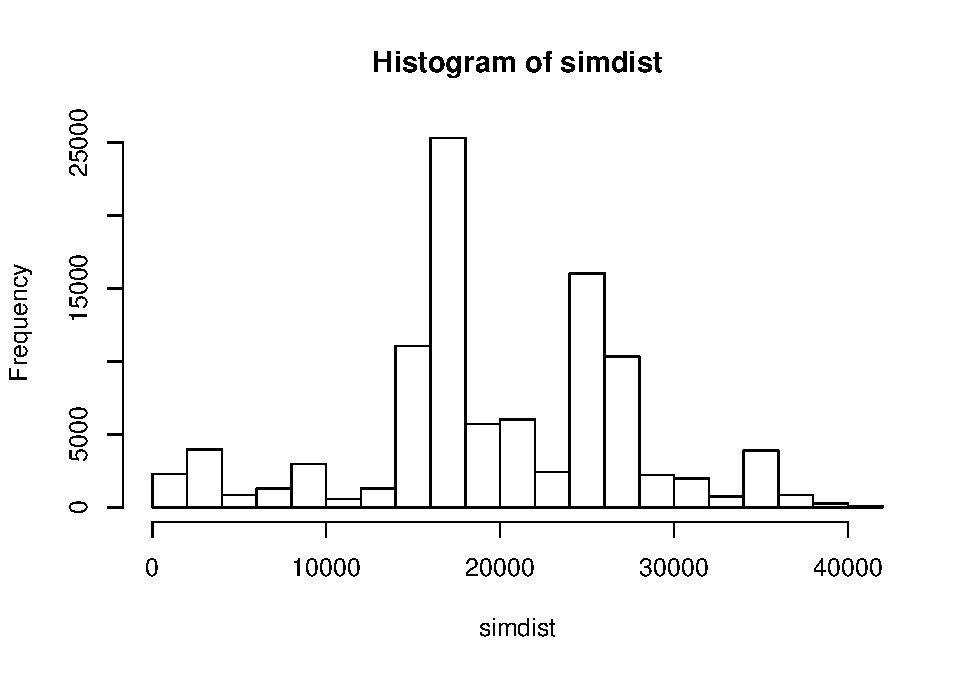
\includegraphics{pvalDist_files/figure-latex/unnamed-chunk-11-1.pdf}

\newpage

\hypertarget{simulate-binary-outcome-per-case-success-failure}{%
\subsection{Simulate binary outcome per case
(success-failure)}\label{simulate-binary-outcome-per-case-success-failure}}

Now we need to simulate binary oucomes upon simulated probabilities
distrbutions for every case x 10000 times. Code:

\begin{Shaded}
\begin{Highlighting}[]
\CommentTok{# VECTOR OF SIMULATED BINARY OUTCOMES UPON SINGLE RANDOM SUCCESS PROBABILITY}
\CommentTok{# FROM EACH DISTRIBUTION OF PROBABILITIES }
\NormalTok{binarySim <-}\StringTok{ }\ControlFlowTok{function}\NormalTok{(distr.p) \{}
        
        \CommentTok{# take by 1 random value from each distribution (for each probability)}
\NormalTok{        rand.each1 <-}\StringTok{ }\KeywordTok{vapply}\NormalTok{(distr.p, }\ControlFlowTok{function}\NormalTok{(x) }\KeywordTok{sample}\NormalTok{(x, }\DecValTok{1}\NormalTok{), }\KeywordTok{numeric}\NormalTok{(}\DecValTok{1}\NormalTok{))}
        
        \CommentTok{# 1 sample from each dist as "success probability" for binary simulation}
\NormalTok{        bin.sim <-}\StringTok{ }\KeywordTok{vapply}\NormalTok{(rand.each1, }\ControlFlowTok{function}\NormalTok{(b) \{}
                \KeywordTok{sample}\NormalTok{(}\DataTypeTok{x       =} \KeywordTok{c}\NormalTok{(}\DecValTok{0}\NormalTok{, }\DecValTok{1}\NormalTok{),}
                       \DataTypeTok{size    =} \DecValTok{1}\NormalTok{,}
                       \DataTypeTok{replace =} \OtherTok{TRUE}\NormalTok{,}
                       \DataTypeTok{prob    =} \KeywordTok{c}\NormalTok{(}\DecValTok{1} \OperatorTok{-}\StringTok{ }\NormalTok{b, b))}
\NormalTok{                \}, }
                \KeywordTok{numeric}\NormalTok{(}\DecValTok{1}\NormalTok{))}
        
        \KeywordTok{stopifnot}\NormalTok{(}\KeywordTok{length}\NormalTok{(distr.p) }\OperatorTok{==}\StringTok{ }\KeywordTok{length}\NormalTok{(bin.sim))}
        \KeywordTok{return}\NormalTok{(bin.sim)}
\NormalTok{\}}
\end{Highlighting}
\end{Shaded}

~

Example of outcome after repeated running for x10 times:

\begin{Shaded}
\begin{Highlighting}[]
\KeywordTok{set.seed}\NormalTok{(}\DecValTok{2}\NormalTok{)}
\KeywordTok{replicate}\NormalTok{(}\DecValTok{10}\NormalTok{, }\KeywordTok{binarySim}\NormalTok{(pmeandist))}
\end{Highlighting}
\end{Shaded}

\begin{verbatim}
##        [,1] [,2] [,3] [,4] [,5] [,6] [,7] [,8] [,9] [,10]
## 0.85      1    1    1    1    1    1    1    1    0     1
## 0.2345    0    1    0    0    0    0    1    1    0     0
## 0.0555    0    0    0    1    0    0    0    0    0     0
## 0.001     0    0    0    0    0    0    0    0    0     0
## 0.35      0    0    0    0    1    0    0    1    0     1
## 0.16      0    0    0    0    1    0    0    0    0     0
## 0.68      0    0    1    1    1    1    1    0    1     1
## 0.4       0    0    0    0    1    0    1    0    1     0
## 0.12      0    0    0    0    0    0    0    0    0     0
\end{verbatim}

\hypertarget{revnues-distribution}{%
\subsection{Revnues Distribution}\label{revnues-distribution}}

Finaly we add everything up. We use 10000 simulated binary outcomes per
each case, combine it with related Opportunity ID revenue and sum all
values to have simulation of Total Revnue. And Repeat x10K Times.

Code:

\begin{Shaded}
\begin{Highlighting}[]
\CommentTok{# SIMULATED TOTAL REVENUE DISTRIBUTION}
\NormalTok{pvalDist <-}\StringTok{ }\ControlFlowTok{function}\NormalTok{(pvec, valvec, }\DataTypeTok{rep =} \DecValTok{10000}\NormalTok{) \{}
        
\NormalTok{        pmeandist <-}\StringTok{ }\KeywordTok{pMeanDist}\NormalTok{(}\DataTypeTok{pvec =}\NormalTok{ pvec)}
        \KeywordTok{stopifnot}\NormalTok{(}\KeywordTok{length}\NormalTok{(pmeandist) }\OperatorTok{==}\StringTok{ }\KeywordTok{length}\NormalTok{(valvec))}
        
\NormalTok{        rsim <-}\StringTok{ }\KeywordTok{replicate}\NormalTok{(rep, \{}
                \CommentTok{# Apply each binary outcome to related revenue}
\NormalTok{                rev <-}\StringTok{ }\KeywordTok{sum}\NormalTok{(valvec }\OperatorTok{*}\StringTok{ }\KeywordTok{binarySim}\NormalTok{(pmeandist))}
                \KeywordTok{return}\NormalTok{(rev)}
\NormalTok{        \})}
        
        \KeywordTok{stopifnot}\NormalTok{(}\KeywordTok{length}\NormalTok{(rsim) }\OperatorTok{==}\StringTok{ }\NormalTok{rep)}
        \KeywordTok{return}\NormalTok{(rsim)}
\NormalTok{\}}
\end{Highlighting}
\end{Shaded}

\begin{Shaded}
\begin{Highlighting}[]
\KeywordTok{set.seed}\NormalTok{(}\DecValTok{1}\NormalTok{)}
\NormalTok{simdist <-}\StringTok{ }\KeywordTok{pvalDist}\NormalTok{(}\DataTypeTok{pvec =}\NormalTok{ src}\OperatorTok{$}\NormalTok{prob, }\DataTypeTok{valvec =}\NormalTok{ src}\OperatorTok{$}\NormalTok{reve, }\DataTypeTok{rep =} \DecValTok{1000000}\NormalTok{)}
\end{Highlighting}
\end{Shaded}

Output head:

\begin{Shaded}
\begin{Highlighting}[]
\KeywordTok{str}\NormalTok{(simdist)}
\end{Highlighting}
\end{Shaded}

\begin{verbatim}
##  num [1:1000000] 23000 10000 18000 27000 29000 28000 16000 29000 26000 9000 ...
\end{verbatim}

Total Revenue Distribution Simulation Histogram:

\includegraphics{pvalDist_files/figure-latex/unnamed-chunk-17-1.pdf}

Mathematical Expectation of Example Dataset is exactly around simulated
mean!:

\begin{Shaded}
\begin{Highlighting}[]
\KeywordTok{sum}\NormalTok{(src}\OperatorTok{$}\NormalTok{reve }\OperatorTok{*}\StringTok{ }\NormalTok{src}\OperatorTok{$}\NormalTok{p)}
\end{Highlighting}
\end{Shaded}

\begin{verbatim}
## [1] 21907.5
\end{verbatim}


\end{document}
